\label{1.4.10}

Let $Y$ be the cuspial cubic curve $y^2 = x^3$ in $\A^2$. Blow up the point $O = (0, 0)$, let $E$ be the exceptional curve, and let $\widetilde{Y}$ be the strict transform of $Y$. Show that $E$ meets $\widetilde{Y}$ in one point, and that $\widetilde{Y} \cong \A^1$. In this case the morphism $\phi: \widetilde{Y} \longrightarrow Y$ is a homeomorphism, but it is not an isomorphism.

\begin{proof}
    We can write $\phi^{-1}[Y] = E \cup \phi^{-1}[Y - 0]$, where $E = \phi^{-1}[0]$ is the exceptional curve. Taking closures, we get $\phi^{-1}[Y] = E \cup \widetilde{Y}$. This is the irreducible decomposition of $\phi^{-1}[Y]$, which is defined in $\A^2 \times \P^1$ by the equations $y^2 = x^3$ and $xu = yt$. If we intersect $\phi^{-1}[Y]$ with some nonempty open subset $U$ we therefore get $(E \cap U) \cup (\widetilde{Y} \cap U)$, which are both irreducible and not contained in each other. We will therefore try to understand how $E$ and $\widetilde Y$ intersect in affine open patches.

    Indeed, let's start with $D(t) = \{t = 1\} \subseteq \A^2 \times \P^1$. This is isomorphic to $\A^3$, and $\phi^{-1}[Y] \cap D(t)$ is given by $V(y^2 - x^3, xu - y)$. It's a simple computation to see that this equals $V(x, y) \cup V(u^2 - x, xu - y)$. The former component is $E \cap D(t)$. The latter, which one can show is irreducible, is therefore $\widetilde Y \cap D(t)$. Thus, $\widetilde Y \cap E \cap D(t) = V(x, y) \cap V(u^2 - x, xu - y)$, which equals $V(x, y, u) = \{0\}$.

    Below is an image of the intersection $\widetilde{Y} \cap D(t)$ in white, along with the exceptional curve $E \cap D(t)$ in yellow. (\ref{fig1.4.1} below)
    \begin{figure}[h]
        \centering
        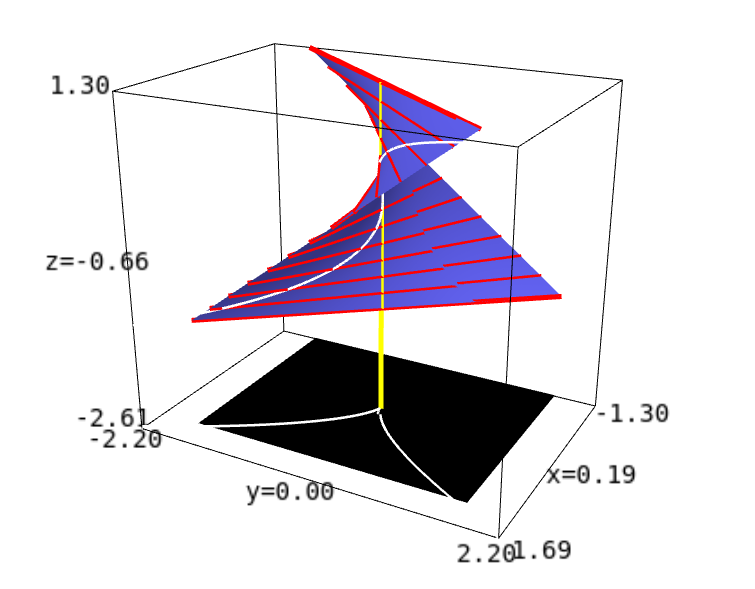
\includegraphics[scale=0.7]{cuspidal-cubic-blowup.png}
        \caption{The blowup of the cuspidal cubic}
        \label{fig1.4.1}
    \end{figure}


    On the other hand, if we intersect with $D(u) = \{u = 1\}$ we get $V(y^2 - x^3, x - yt) = V(x, y) \cup V(1 - yt^3, x - yt^3)$. The intersection of these is $V(x, y, 1 - yt^3, x - yt) = V(x, y, 1) = \emptyset$.

    Thus, we have computed the intersection $\widetilde Y \cap E = (0, 0, [1 : 0])$. This, additionally, shows that $\widetilde Y = \phi^{-1}[Y - 0] \cup \{(0, 0, [1 : 0])\}$. The parametrization $\A^1 \longrightarrow Y$ via $t \mapsto (t^2, t^3)$ yields a parametrization $\A^1 - 0 \longrightarrow \phi^{-1}[Y - 0]$ via $t \mapsto (t^2, t^3, [t^2 : t^3])$. We can extend this to $\A^1$ via $0 \mapsto (0, 0, [1 : 0])$. I claim that this is an isomorphism of varieties $\A^1 \longrightarrow \widetilde Y$. It is given by maps $\A^1 \longrightarrow \A^2$ via $t \mapsto (t^2, t^3)$ and $\A^1 \longrightarrow \P^1$ via $t \mapsto [1 : t]$, so it's at least a morphism of varieties. Its inverse is given by the projection $Y \longrightarrow \P^1$, whose image consists of those elements of the form $[1 : t]$, which maps isomorphically to $\A^1$ via $[1 : t] \mapsto t$.
    
    The projection back down to $Y$ returns us to the usual parametrization of $Y$, which is not an isomorphism but is a homeomorphism.

    NOTE: I'm not completely happy with the rigor here.
\end{proof}
